% Blockchain Designs for In-Space Economies
%
% \textbf{TODO}: Check for more up-to-date AIAA journal template, and for any specific ARC JIS template.
% This paper uses the AIAA Basic template, which seems to suit our needs.
%
% `template_basic.tex' - A bare-bones example of using the AIAA class.
%                        For a more advanced usage, see `template_advanced.tex'.
%
% Typical processing for PostScript (PS) output:
%
%  latex template_basic
%  latex template_basic   (repeat as needed to resolve references)
%
%  xdvi template_basic    (onscreen draft display)
%  dvips template_basic   (postscript)
%  gv template_basic.ps   (onscreen display)
%  lpr template_basic.ps  (hardcopy)
%
% With the above, only Encapsulated PostScript (EPS) images can be used.
%
% Typical processing for Portable Document Format (PDF) output:
%
%  pdflatex template_basic
%  pdflatex template_basic      (repeat as needed to resolve references)
%
%  acroread template_basic.pdf  (onscreen display)
%
% If you have EPS figures, you will need to use the epstopdf script
% to convert them to PDF because PDF is a limmited subset of EPS.
% pdflatex accepts a variety of other image formats such as JPG, TIF,
% PNG, and so forth -- check the documentation for your version.
%
% If you do *not* specify suffixes when using the graphicx package's
% \includegraphics command, latex and pdflatex will automatically select
% the appropriate figure format from those available.  This allows you
% to produce PS and PDF output from the same LaTeX source file.
%
% To generate a large format (e.g., 11"x17") PostScript copy for editing
% purposes, use
%
%  dvips -x 1467 -O -0.65in,0.85in -t tabloid template_basic
%
% For further details and support, read the Users Manual, aiaa.pdf.
%
% This software is released under the terms of the LaTeX Project Public
% License.  Copyright (C) 2004 by Bil Kleb, Bill Wood, and Erich Knausenberger.


\documentclass[]{aiaa-tc}% insert '[draft]' option to show overfull boxes

% Author-specific packages
\usepackage[breaklinks=true]{hyperref}
\hypersetup{colorlinks, citecolor=green, filecolor=black, linkcolor=blue, urlcolor=blue }
\usepackage{mathpazo}
\newcommand{\rpm}{\raisebox{.2ex}{$\scriptstyle\pm$}} % for +- character
\usepackage[shortlabels]{enumitem} % for lettered lists
\usepackage[colorinlistoftodos]{todonotes} % TODOs
% End author-specific packages

 \title{Blockchain Properties for Near-Planetary, Interplanetary and Metaplanetary Space Domains}

% \textbf{TODO}: Not ordered yet
 \author{
  David Hyland-Wood%
    \thanks{PegaSys, ConsenSys Australia, Brisbane, Queensland, Australia}
    \thanks{School of Information Technology and Electrical Engineering, The University of Queensland, Brisbane, Australia}
    \thanks{AIAA Member}\\
  \and Peter Robinson\thanksibid{1} \thanksibid{2}
  \and Chris Lewicki%
   \thanks{ConsenSys Space, Redmond, Washington, USA}
   \thanksibid{3}
  \and Christopher Hare\thanksibid{1}
  \and Roberto Saltini\thanks{PegaSys, ConsenSys Australia, Sydney, New South Wales, Australia}
  \and Sandra Johnson\thanksibid{1}
  	\thanks{ARC Centre of Excellence for Mathematical and Statistical Frontiers, Queensland University of Technology, Brisbane, Australia}
  \and Brett Henderson\thanksibid{1}
 }

 % Data used by 'handcarry' option if invoked
 \AIAApapernumber{YEAR-NUMBER}
 \AIAAconference{Conference Name, Date, and Location}
 \AIAAcopyright{\AIAAcopyrightD{YEAR}}

 % Define commands to assure consistent treatment throughout document
 \newcommand{\eqnref}[1]{(\ref{#1})}
 \newcommand{\class}[1]{\texttt{#1}}
 \newcommand{\package}[1]{\texttt{#1}}
 \newcommand{\file}[1]{\texttt{#1}}
 \newcommand{\BibTeX}{\textsc{Bib}\TeX}
 
 \hyphenation{block-chain}
 \hyphenation{block-chains}
 \hyphenation{econ-o-mies}

\begin{document}

\maketitle

\begin{abstract}
Blockchain technologies have demonstrated new and interesting ways to construct terrestrial economies, including the well-known public cryptocurrencies, but also as means to facilitate business-to-business (B2B) and business-to-consumer (B2C) transactions. Some have recently proposed uses for blockchains in space. This paper identifies desirable blockchain properties that could be used to construct future in-space economies.

Three general economic domains are anticipated, each with their own communications limitations that drive the selection of applicable blockchain properties: Operations in orbits around planetary bodies where realtime communication is possible (e.g. within cislunar space around Earth or cisdeimotic space around Mars), operations across interplanetary space between spheres of influence where pseudo-realtime communication is possible (e.g. Earth-Mars or Earth-asteroids), and operations in metaplanetary space within the Solar system but beyond the limit of pseudo-realtime communication. Blockchain properties are suggested for each domain, with a focus on the selection of blockchain consensus algorithms. Evaluation is performed on the readiness of extant technologies to operate in each domain.
\end{abstract}

\section*{Nomenclature}
\begin{tabbing}
  XXX \= \kill% this line sets tab stop
  $b$ \> Average block size, a function of the number of transactions per block \\
  $n$ \> The number of blockchain nodes in a network \\
 % $N_{n}$ \> The total number of participating blockchain nodes \\
  %$v$ \> A validator participating in a blockchain consensus protocol \\
  %$N_{v}$ \> The total number of participating validators \\
  %\textit{Subscript}\\
  %$i$ \> Variable number \\
 \end{tabbing}

%%%%%%%%
% SECTION % 
%%%%%%%%
\section{Introduction}

Blockchain technologies have demonstrated new and interesting ways to construct terrestrial economies, including the well-known public cryptocurrencies, but also as means to facilitate business-to-business (B2B) and business-to-consumer (B2C) transactions. This paper identifies desirable blockchain properties that could be used to construct in-space economies.

An in-space blockchain can serve as a natural basis for an in-space economy due to the ability of a blockchain to establish a trust environment of peers in consensus, and a facility to execute smart contracts when and if certain (perhaps difficult) activities are provably undertaken. Many, although certainly not all, of the smart contracts implemented to date execute economic agreements; we suggest that general trend is likely to continue into activities in space. It is therefore not too early to think about the properties required by an in-space blockchain.

Spacecraft face challenges not present with terrestrial computing systems. Due to launch costs, limitations in means of making or carrying electrical power, and the challenges of dissipating heat in a vacuum, available power and computation capabilities are much more limited on spacecraft than they are terrestrially. Moreover, computation, non-volatile and volatile memory options are constrained by the limits imparted on microelectronics in order to operate reliably in hard radiation environments.  Spacecraft have to cope with great distances leading to significant light speed delays in communication, and occasional inability to get a line-of-sight to communications nodes in the same network.  Such distances create challenges in data integrity verification, communications acknowledgements, store-and-forward and multi-path considerations, compounded by free-space path losses resulting in bandwidth constraints. This swathe of challenges introduced by spacecraft necessitates the invention of new kinds of blockchains to serve those needs.

Three general economic domains are anticipated, each with their own communications limitations that drive the selection of applicable blockchain properties: Operations in orbits around planetary bodies where realtime communication is possible (e.g. cislunar space within the orbit of Earth's moon or ``cisdeimotic'' space within the orbit of Mars' moon Deimos), operations across interplanetary space between spheres of influence where pseudo-realtime communication is possible (e.g. Earth-Mars or Earth-asteroids), and operations in metaplanetary space within the Solar system but beyond the limit of pseudo-realtime communication. Blockchain properties are suggested for each domain, with a focus on the selection of blockchain consensus algorithms. Evaluation is performed on the readiness of extant technologies to operate in each domain.

This paper will review current implementations and proposals for blockchain uses in space (Section \ref{sec:litreview}). We will then determine desirable blockchain properties for the three domains (Section \ref{sec:desiredproperties}): 
\begin{enumerate}[(a)] % list of style (a), etc.
\item Near-planetary space
\item Interplanetary space
\item Metaplanetary space
\end{enumerate}

Figure \ref{f:fig1-toroid-of-interest} illustrates the three domains with a toroid of interest for medium-term in-space economies. The toroid is defined for convenience with an inner edge at the Earth-Sun $L_{1}$ point, an outer edge at the outer limit of the main asteroid belt at the strong Kirkwood gap at 3.27 AU from the Sun (where asteroids are in a 2:1 mean-motion resonance with Jupiter, also known as the Hecuba gap), and with upper and lower bounds $\rpm 20$ degrees from Sun center above and below the plane of the ecliptic.

Finally, we will report our conclusions and suggest directions for future work.


%%%%%%%%
% SECTION %
%%%%%%%%
\section{Literature Review}\label{sec:litreview}

The application of blockchain technologies to space operations has recently attracted significant attention. At least two companies currently provide some form of blockchain operations in Earth orbit: SpaceChain Foundation\footnote{https://spacechain.com/} has launched two CubeSats into LEO, operating nodes of a QTum blockchain, and has deployed a multi-signature cryptocurrency wallet experiment via Nanoracks on the International Space Station. Blockstream\footnote{https://blockstream.com/} leases bandwidth on five existing GEO telecommunications satellites to broadcast the Bitcoin data stream.

Researchers in several countries have proposed future uses of blockchains in space including:
\begin{itemize}
\item use as a property registry\cite{beldavs_blockchains_2016}
\item for identity management, especially for protection against cyber attacks \cite{yu_blockchain_2019,xu_exploration_2019}
\item to  ``facilitate on-orbit satellite communication data integrity and security''\cite{molesky_blockchain_2018} (i.e. secure command and control)
\item to reduce ``manual intervention in monitoring and control''\cite{jennath_distributed_2019}
\item in ``tracking various components of vehicles''\cite{jennath_distributed_2019}
\item as a component of ``smart services for space traffic management''\cite{skobelev_towards_2018}
\item as a means to coordinate the fulfillment of a desired operation carried out by many individual spacecraft\cite{mandl_bitcoin_2017}
\end{itemize}

Researchers with government or military connections in China, Russia and the United States are actively investigating uses of blockchains for access security and data integrity of Earth-orbiting satellites. Published Chinese military interest seems to be focused on preventing ``cyber \& physical attacks'' against space assets\cite{yu_blockchain_2019}, and to allow ``multiple departments to participate in the maintenance and update of equipment status''\cite{yu_situational_2019}. The Roscosmos State Corporation for Space Activities in Russia is developing a ``digital platform for control spacecrafts'' [sic] and for ``use of ground stations'' focused on the ``Roskosmos orbital group'' of satellites\cite{skobelev_towards_2018}. It has been suggested that ``the US military has taken a fancy to the anonymity of blockchain in recording transactions, and has begun to expand to the field of intelligence gathering to achieve covert targeted payments for incentive personnel.'' [sic]\cite{yu_situational_2019}. Mandl, at NASA Goddard Space Flight Center, has proposed using smart contracts on blockchains to create a ``Remote Sensing as a Service'' offering\cite{mandl_bitcoin_2017}. In Mandl's conception, a single Earth observation requirement could be obtained by multiple platforms conducting multiple observations under a variety of conditions until a desired goal is achieved.
\subsection{Applicability of Blockchain Technology}
The space-based communications security use cases above bear resemblance to similar terrestrial use cases for communication security of air traffic control systems\cite{reisman_air_2019} and bear significant resemblance to issues encountered in distributed Internet of Things networks (e.g. \cite{dorri2017lsb, dorri2019mof}).

The first question that we ought to answer is whether a blockchain is a legitimate solution for these use cases. We therefore begin by ensuring that we match stated domain requirements to a theoretical framework for blockchain applicability. Several researchers (e.g. \cite{wust_gervais_2017,xu_design_2019}) have proposed decision trees to help determine the applicability of blockchains to particular domains. We will follow W\"{u}st and Gervais\cite{wust_gervais_2017} to suggest blockchain properties that could be used to satisfy the goals for some space-related use cases. W\"{u}st and Gervais determined blockchains are best used when all of the following criteria are met: Storage of state is required, the system has multiple writers, a trusted third party is not appropriate or not available, or a controlling third party's network cannot be trusted due to potential intrusion, issues of slow latency or low throughput are acceptable, and a centrally managed system is inappropriate or not practical.

W\"{u}st and Gervais continue by noting that a permissionless blockchain should be used when the above conditions are met and not all writers are known, and a permissioned blockchain should be used when the above conditions are met and all writers are known. Using their guidelines, we find that an in-space economy where the participants include multiple spacecraft controlled by multiple operators which may change over time, matches the criteria for a blockchain. There is certainly no agreed arbiter of a future in-space economy at this time, and it would seem reasonable to question whether one could arise due to the currently rapid decentralization of spacecraft ownership.

The small number (in distributed computing terms) of extant and expected spacecraft could allow for a ``closed economy'' wherein participants may be well known and require either permission or at least registration to join or leave a network. Such permissioned networks trade off software complexity (especially the need to manage cryptographic keys) with simpler runtime requirements (due to the ability to know, and therefore to some degree trust) participants.

Several of us (Hyland-Wood, Robinson, Saltini, Johnson and Hare) have previously outlined how permissioned blockchains may be used as trust systems when a central authority may not be able to be trusted, as is the case when the underlying network, network services and/or user accounts may have been compromised.\cite{hyland-wood-icssc2019}. We proposed using such a system to secure spacecraft command channels in the presence of cybersecurity attacks against networks that control spacecraft.

It also seems appropriate to apply blockchains to the building of in-space economies because they have been successfully used to build terrestrial economies. As noted by Beldavs\cite{beldavs_blockchains_2016}, ``Central to the economy is money and rules for transacting business, as well as institutions that facilitate business activity such as banks.''. Blockchains can theoretically fulfill all of those criteria. The two largest, and earliest, public blockchains Bitcoin\cite{nakamoto_bitcoin_2008} and Ethereum\cite{buterin_ethereum_2013,wood_ethereum_2014} have both created usable currencies (in spite of their volatile prices), defined rules for transacting business, and included smart contract functionality\cite{szabo_smart_1994} that may be used to facilitate business activity.

Beldavs\cite{beldavs_blockchains_2016} further suggests that the establishment of property rights and the use of a property registration system are necessary conditions for the establishment of an in-space economy\cite{beldavs_blockchains_2016}. He asserts that any future property rights over space resources ``will need to be compliant with the Outer Space Treaty that excludes conventional real property whose ownership rights are granted by a sovereign state.''. While he is correct in quoting Article II of the Outer Space Treaty\cite{UNCPUOS_1967} ``Outer space, including the moon and other celestial bodies, is not subject to national appropriation by claim of sovereignty, by means of use or occupation, or by any other means'', it is currently unclear that the Outer Space Treaty will survive large-scale economic activities in space, nor that those with fortunes to be made will voluntarily bind themselves to it. The approach generally taken in the field of economics, i.e. empirically considering the choices humans make given incentives, would tend to indicate that exactly the opposite may happen. The Outer Space Treaty is likely to be replaced by subsequent agreements that both allow and foster an in-space economy. Others have noted that the current legislative structures focus on ``the non-militarisation of space, the promotion of scientific endeavours and the mitigation of orbital debris. However, the legislative framework does not presently anticipate the use of orbital planes in LEO for commercial actors or the management of orbital shells for LEO.''\cite{green_mitigation_2018}. Effective ``natural monopolies'' could therefore form (in the absence of new legislation or treaties) by commercial dominance of particularly useful orbital shells. The anticipated dominance of orbital shells by SpaceX Starlink, OneWeb, and Amazon Kuiper communications satellites are topical examples of such effective monopolies, and a reason to suggest that the current nation-based legislative environment (as defined in Article VI of the Outer Space Treaty\cite{UNCPUOS_1967}) is unstable due to the rise of commercial space interests.

Israel has proposed that a $\mathit{lex\; mercatoria}$-like system may form in space, similar to the economies that developed between companies operating away from their home countries during the Age of Exploration\cite{israel_space_2019}. Blockchains, with their decadal history of performing $\mathit{lex\; mercatoria}$-like operations, seem to be a reasonable fit for the likely conditions.

\subsection{Challenges with Deploying Blockchains in Space}
The second question that we ought to answer is whether blockchains can actually be deployed in space.
This because the space environment imposes limitations and presents challenges that are quite different from the air-conditioned, high-bandwidth terrestrial environments where early blockchain technologies were developed.

Properties of the near-Earth orbital space environment that impose additional limitations on blockchain technologies include:
\begin{itemize}
\item \textit{computing system resources}. Limitations include computational capabilities, memory\cite{CCSDS_2007} and storage\cite{yu_blockchain_2019}. Electrical power available to be dedicated to computation is also generally limited, as is the ability of a spacecraft thermal control system to maintain a computing system within operational limits.
\item \textit{environmental conditions.} Limiting environmental conditions include ``noisy, bandwidth limited, asymmetrical, and interrupted communications links''\cite{CCSDS_2007}.
\end{itemize}

Communication delays may be compounded by mission-specific requirements. For example, some space missions include ``a requirement for early access to transferred data regardless of its quality''\cite{CCSDS_2007}. Choices between early, low-quality data (including ``lossy'' data and/or partial data sets) and later higher-quality data, coupled with ever-changing relative positions and thus propagation delays, possibilities for communications blackouts due to positions, power availability, errors, or other factors combine to make specific situations unique.

The farther from Earth one operates in space, the more propagation delays affect communications. Such delays are an important facet of space systems design\cite{CCSDS_2007,yu_blockchain_2019}. Delays are a particularly important design criterion for blockchain consensus algorithms because timeouts are often used to determine when consensus cannot occur, and to denote error conditions.

It is straightforward to determine propagation delays in radio communication if one knows the distances involved since radio waves travel at the speed of light. Propagation delays between Earth and Mars can vary between as little as three and a half minutes each way 
to
 as much as twenty four minutes each way depending on the relative positions of the two planets in their orbits. Delays to the outer edge of the main asteroid belt, known as the outer Kirkwood gap, can reach over thirty five minutes in each direction when a spacecraft at the outer Kirkwood gap is in conjunction with Earth. Additionally, available communications bandwidth is degraded as propagation losses increase. It is clear that consensus algorithms used on blockchains for space operations even within the inner Solar System (that narrow toroid defined by Earth, the Moon, Mars, and the main asteroid belt, as illustrated in Fig. \ref{f:fig1-toroid-of-interest}) will need to treat such lengthy propagation delays as a key design criterion.

\begin{figure}[htb]% order of placement preference: here, top, bottom
 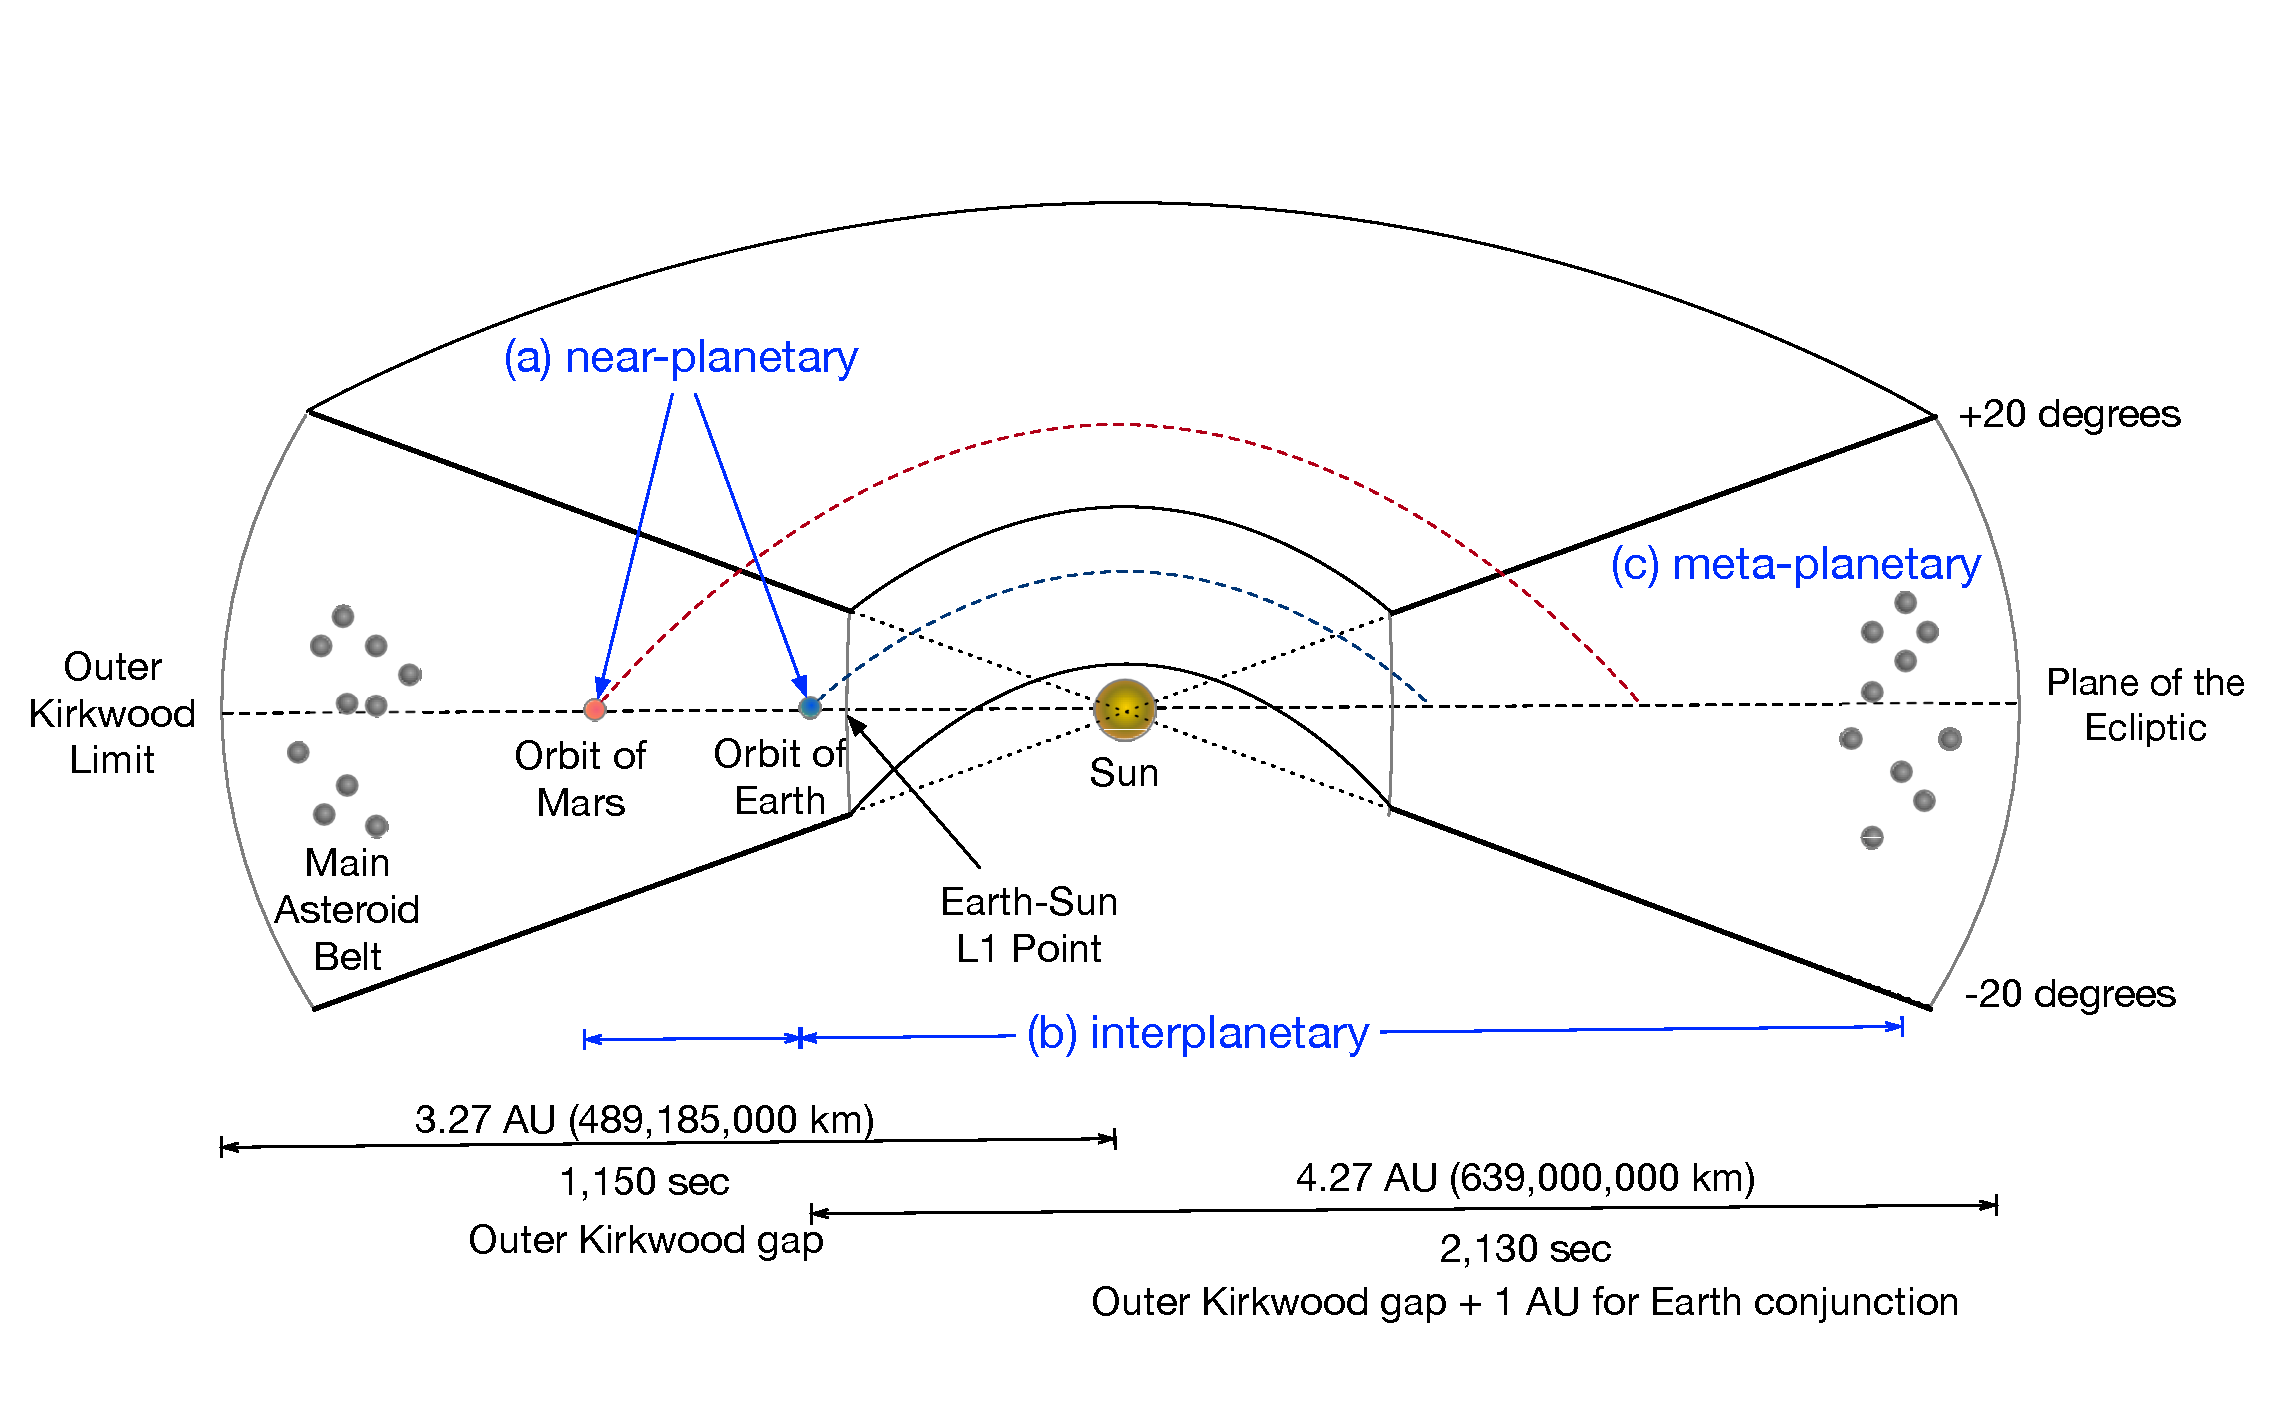
\includegraphics{figures/fig1-toroid-of-interest}
 \caption{A toroid of interest for a near-future in-space economy}
 \label{f:fig1-toroid-of-interest}
\end{figure}

Spacecraft communicating with controllers solely via relays require certain adjustments to be made to their designs to allow them to maintain fault-tolerant operations\cite{lewicki_phoenix_2006}. Those adjustments include designs that anticipate and automatically handle a greater number of communications disruptions due to the relays, and designs allowing spacecraft commands to be sent ``in the blind'' with automatic handling of inappropriate commands on the spacecraft itself. Such considerations provide important design criteria for any distributed computing scenario.

Some of the limitations noted above are physical and so immutable over time, such as light speed delays, and physical lines of sight. Others are dependent on the state of technology, and are thus likely to change, such as compute, memory, storage, power generation and heat rejection. Economic transactions in space are similarly most likely to start as small in message sizes, bandwidth usage, and in absolute number, but may reasonably be expected to grow by orders of magnitude as an in-space economy develops and becomes a mainstream activity. Any proposed technological solution treating these requirements as design criteria should therefore take into account those that might change and those that are fixed.

Difficulties in communication with spacecraft have been experienced for decades, and solutions have been implemented in depth. Newer techniques have included experiments with lasers to increase the directionality, and hence the available bandwidth, of direct spacecraft communications. However, regardless of available bandwidth, the limitations above will continue to dominate communication systems. The Consultative Committee for Space Data Systems, an international cooperative body to create space data standards, has been working on this problem since the 1980s. The CCSDS File Delivery Protocol (CFDP) has provided a standard file transfer protocol for transmitting data to spacecraft since 2002\cite{CCSDS_2007}. CFDP supports both unreliable and reliable file-oriented data transfer. While these standards are increasingly comprehensive, spacecraft flight software implementations of them are almost always partial (often with cost/implementation-convenient violations of the standards), and not yet available in open-source repositories.

Data transfer over unreliable communication links can nevertheless be made reliable by the use of various error-detection and error-correction schemes. NASA's deep space missions and some commercial telecommunications satellites are currently using forward error-correction Turbo codes\cite{berrou_near_1993} for this purpose.  Data security considerations for deep space missions has thus far been minimal, as the physical barriers to interacting with these assets are severe.

A useful approach to abstract above current Internet networking protocols for an ``interplanetary Internet'' was developed to ensure delivery of file-oriented data in a ``postal model of communication''\cite{burleigh_delay-tolerant_2003}. This email-like functionality over communications systems with very high degrees of transmission latency was specifically aimed at deep space communications challenges. The effort was confusingly known as Disruption Tolerant Networking at the funding agency, the U.S. Defense Advanced Projects Research Agency (DARPA). Unfortunately, the proposals did not progress to the Standards Track of the Internet Engineering Task Force where they were originally published, and the original research group disbanded around 2005. New work on Delay/Disruption Tolerant Networking currently continues at NASA\cite{mahoney_disruption_2016}.

Prototypical implementations of Delay/Disruption Tolerant Networking demonstrated successful operation with delays lasting up to sixty minutes. Round-trip communication delays within the Earth-Moon-Mars-asteroid belt toroid suggest the motivating factor in testing delays of that period.

The notional ``heart'' of a blockchain is its consensus algorithm. A blockchain consensus algorithm defines the steps necessary for blockchain participants to agree on information to be added to the distributed ledger. It is how the nodes in the network agree (come to consensus on) the next block to be added to the chain\cite{hyland-wood_future_2018}.

Existing blockchain consensus algorithms have been recognized by many as limiting the applicability of blockchains to space operations\cite{yu_blockchain_2019,yu_situational_2019,mandl_bitcoin_2017,molesky_blockchain_2018,xu_exploration_2019}. It is particularly important to recognise the engineering tradeoffs inherent in increasing power consumption on spacecraft\cite{lyke_energy_2017}.

Several researchers have suggested the applicability of Ethereum as a possible blockchain framework (e.g. \cite{israel_space_2019}), but noted that the consensus algorithms currently used on the public production Ethereum blockchain (known as ``Ethereum MainNet'') are inappropriate for use in space operations\cite{molesky_blockchain_2018,xu_exploration_2019,mital_blockchain_2019}. Neither the traditional proof of work (PoW) algorithm nor the forthcoming proof of stake (PoS) consensus algorithm used on Ethereum MainNet or its public test networks provide the properties needed for space operations. For example, Ethereum PoW is intentionally designed to be computationally intensive, and Ethereum PoS relies upon the blockchain having an economically meaningful cryptocurrency to be used for internal operations. Neither algorithm would cope well with blockchain nodes operating in a significantly time-delayed, or low-availability network environment.

Changing the consensus algorithm of an Ethereum system creates a blockchain that is incompatible with Ethereum MainNet, at least under the current state of the art. Those taking this path (e.g. the Enterprise Ethereum Alliance and its members, and those researchers cited in the previous paragraph) are thus proposing ``private'' or ``enterprise'' Ethereum blockchains with consensus algorithms and perhaps other properties they deem appropriate for operations in their contexts.

Three groups have suggested the Practical Byzantine Fault Tolerance (PBFT) algorithm\cite{castro_practical_1999} as a possible consensus algorithm for near-Earth orbital space operations\cite{yu_blockchain_2019,molesky_blockchain_2018,mital_blockchain_2019}. One presumes those researchers meant to suggest PBFT as modified for use as a blockchain consensus algorithm, e.g. Istanbul Byzantine Fault Tolerance\cite{lin_istanbul_2017}, since PBFT was not itself defined with blockchains in mind. The PBFT family of consensus applications are a 
possible, but imperfect, fit for orbital space operations given their reliance on time and connectivity as critical algorithmic components. Timeouts resulting from communications delays, occultation, radio interference, and other communication disruptions are all too common with spacecraft, but are used to determine error conditions in the PBFT family of consensus algorithms. PBFT algorithms would be an even less perfect fit for deep space operations where such communication disruptions are routinely expected. PBFT message sizes also tend to be large in practice, which work against the bandwidth, processing, and storage capabilities of most extant and proposed spacecraft. However, blockchains using PBFT algorithms located terrestrially or in orbits with certain restrictions (i.e. those with continuous communication ability, including those in geosynchronous orbits and those in LEO/MEO orbits with communications relays) may still be a reasonable component of integrated space systems.


%%%%%%%%
% SECTION %
%%%%%%%%
\section{Desired Blockchain Properties}\label{sec:desiredproperties}

Several logical blockchain-spacecraft relationships are possible, and each relationship implies a different overall systems architecture. Figure \ref{f:fig2-blockchain-arch} illustrates four possible architectural relationships between a blockchain and a spacecraft. A spacecraft may act as a regular blockchain node (a), or as a mining node, sometimes also known as a writer or a 
validator
 (b). A spacecraft may simply read information from a blockchain (c) or request transactions be written to a blockchain (d). These possible relationships imply very different computation capacity and radio bandwidth onboard spacecraft, especially due to overall message traffic and average message size. We will suggest a blockchain-spacecraft relationship suitable for each of the target domains.

\begin{figure}[htb]% order of placement preference: here, top, bottom
 \centering{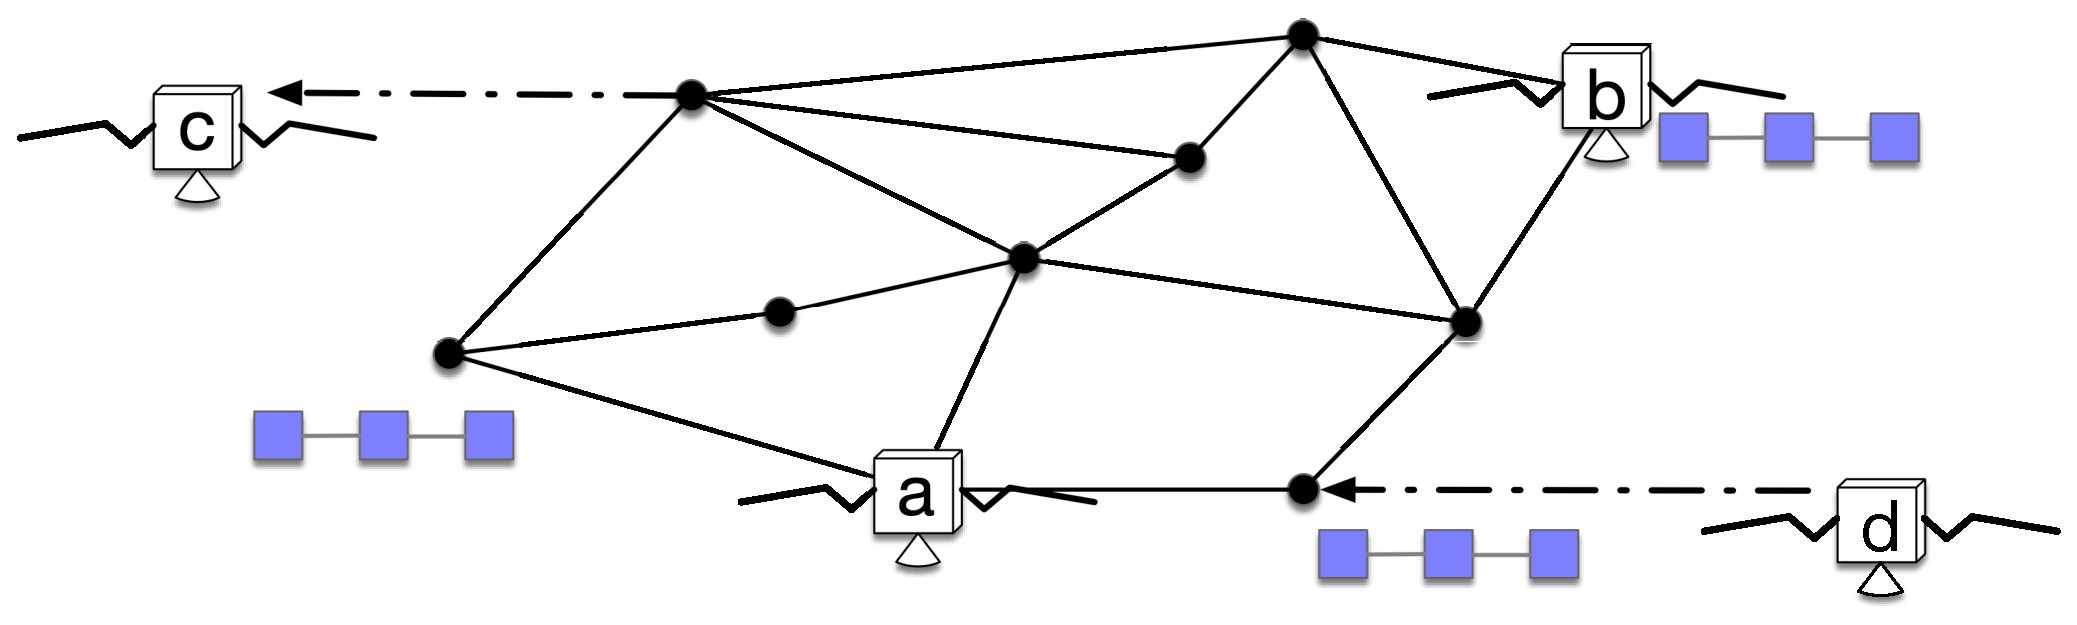
\includegraphics[width=300px,keepaspectratio]{figures/blockchain-arch}} 
 \caption{Possible blockchain-spacecraft relationships}
 \label{f:fig2-blockchain-arch}
\end{figure}

Table \ref{t:tab1-spacecraft-rels} compares the possible relationships between spacecraft and blockchains in terms of the relative amount of message traffic necessary to participate in each manner, and the relative degree to which onboard software would need to change to support blockchain operations of each type. By far the most compelling relationship between a spacecraft and a terrestrial blockchain is for the spacecraft to read information from the blockchain, as illustrated in Fig. \ref{f:fig2-blockchain-arch}(c) and compared in Table \ref{t:tab1-spacecraft-rels}. The costs for such read operations are minimal in terms of both message traffic and the degree of software changes. Most existing spacecraft do not have the computational capability to operate a blockchain node, although that restriction seems likely to ease as newer compute buses become space qualified.

\begin{center}
\begin{table}
\caption{Comparison of possible blockchain-spacecraft relationships}
 \label{t:tab1-spacecraft-rels}
\begin{center}
\begin{tabular}{lll}
\hline
Relationship    & Message traffic to/from satellite & Changes needed to onboard software \\
\hline
(a) Regular node      & High    & High      \\
(b) Mining node       & High     & High      \\
(c) Read-only       & Low     & Low-Medium      \\
(d) Write request & Low      & Medium       \\
\hline
\end{tabular}
\end{center}
\end{table}
\end{center}


\subsection{Near-Planetary Economies}

Terrestrial distributed computing systems may choose to access sub-millisecond timing signals available via global navigation satellite systems (GNSS) or atomic clock broadcast signals. Spacecraft in Earth orbit can similarly leverage such signals to develop and maintain a common sense of time, even when relativistic corrections must be made. Spacecraft in Earth orbit also naturally suffer less from extreme time delays or communication loss than those in deep space. 

With a common notion of time and relatively short time delays, devices within cislunar space can effectively join terrestrial blockchains that use time as an intrinsic part of their consensus algorithms. Developing similar systems around Mars (say, within cisdeimotic space) will require similar infrastructure to that used around Earth. One tradeoff that must be made is the limitations imposed by light speed delays on block creation speed. That is probably acceptable as long as the number of space-to-space transactions is relatively small. 

It is possible, and probably preferred, to treat most orbiting spacecraft as edge devices as opposed to expecting them to run blockchain node software. In such a scenario, spacecraft may read transactions from, or propose transactions to, a blockchain operated terrestrially. Blockchain nodes on spacecraft are anticipated to remain special-purpose devices deployed on few spacecraft for some time to come.

\subsubsection{Consensus Algorithm Selection for Near-Planetary Space}

Blockchain consensus protocols build on decades of experience creating consensus in distributed computing systems. The most commonly used families of consensus protocols include the proof of work (PoW) algorithms used by the public Bitcoin and Ethereum networks, the proof of stake (PoS) algorithms such as the Ethereum network is attempting to migrate to using, and proof of authority (PoA) algorithms used in private, consortium or ``enterprise'' blockchains where key participants are known.

Neither PoW nor PoS algorithms provide the properties needed for space system operations. All PoW algorithms are intentionally designed to be computationally or memory intensive. It is clearly undesirable for spacecraft to perform unnecessary computation, especially when those computations may not result in a successful transaction. PoS algorithms rely upon the blockchain having an economically meaningful cryptocurrency to be used for internal operations. We suggest the PoA family of algorithms have several properties appropriate for near-planetary and interplanetary scenarios, including agreement on a single chain of transactions and thus immediate finality of each block.

PoA protocols may be conveniently separated into those that guarantee immediate finality of created blocks, those that guarantee eventual finality and those that do not guarantee finality. A block is said to be final only if it has been added to the blockchain of an honest node and both its position and content may not be changed under any future circumstance (e.g. a network fork, or a rebalancing of the blockchain at a later time). A blockchain consensus protocol provides immediate finality only if any block is final as soon as it is added to the blockchain provided that there are no more faulty nodes than the maximum threshold allowed by the protocol. In other words, immediate finality guarantees that the blockchain cannot fork. A blockchain consensus protocol guarantees eventual finality if blocks become final only after they have been on the chain for a ``sufficiently long'' time. In the case that blocks added to the chain never become final, such as in the Clique PoA protocol\cite{Szilagyi-Clique}, then the consensus protocol is said not to guarantee finality.

Another property to be considered when choosing PoA protocols, and consensus protocols more generally, is whether they are tolerant to nodes that 
 act maliciously, 
are faulty, or suffer communications failures. 
 Such nodes are commonly called Byzantine\cite{lamport1982byzantine}. The ability of a network to correctly operate in the presence of Byzantine nodes is called Byzantine fault tolerance (BFT).

Finally, the type of network that a consensus protocol is designed for must be considered. Networks can be divided into three types: synchronous, asynchronous and partially synchronous\cite{dwork1988consensus}. The maximum message delay in synchronous networks is bounded by a known amount of time, and unbounded in asynchronous networks. In partially synchronous networks, either the maximum message latency is finite but unknown or the network is guaranteed to reach a state of synchrony in a finite but unknown time after experiencing an initial state of asynchrony.

We argue that the properties of immediate finality, BFT and the ability to operate on partial synchronous networks are very compelling features for space system operations because they allow for immediate reads of the information known to be on the chain, provide a high level of security and allow for patchy communication which is usually the case for space communication. The Enterprise Ethereum Alliance is considering adoption of immediate finality and BFT in their client standard\cite{eea-enhancedbft}.

PoA protocols that provide immediate finality and Byzantine fault tolerance include Honey Badger\cite{Miller_Xia_Croman_Shi_Song_2016}, Tendermint\cite{Buchman_Kwon_Milosevic_2018}, DBFT (Democratic BFT)\cite{Crain_Gramoli_Larrea_Raynal_2018}, and IBFT 2.0\cite{saltini-ibft2}. Table \ref{t:tab2-poa-algos} summarizes the key properties of these protocols, and indicates our choice of IBFT 2.0 as most appropriate for the near-planetary domain due to its ability to deal with lost messages. A more complete evaluation of these and other PoA protocols is available.\cite{hyland-wood-icssc2019}

\begin{center}
\begin{table}
\caption{Proof of Authority Consensus Algorithms with Immediate Finality and Byzantine Fault Tolerance}
 \label{t:tab2-poa-algos}
\begin{center}
\begin{tabular}{llll}
\hline
Algorithm    & Message traffic to reach consensus & Average message size & Resilience to lost messages \\
\hline
Honey Badger      & O($n^{2}$)    & O(b)   & No   \\
Tendermint       & O($n^{2}$)     & O(b)  & No      \\
DBFT       & O($n^{2}$)     & O(b)  & No      \\
IBFT 2.0 & O($n^{2}$)      & O(b)  & Yes       \\
\hline
\end{tabular}
\end{center}
\end{table}
\end{center}


\subsection{Interplanetary Economies}

Deep space probes today typically act as edge nodes in a CFDP network. They check in directly with Earth as a routine part of their operations. These direct-to-Earth communications may one day yield to communication with other regional centers, such as a Martian outpost or asteroid mining operations, as part of a more diffuse interplanetary network.

We must anticipate that multiple hub nodes will evolve at areas of exceptional deep space activity, such as Lunar, Mars and asteroid operations, and eventually settlements at each and economic encounters between them. Such networks are likely to be complicated as some nodes implement the ability to relay or even foster direct spacecraft-to-spacecraft communication, thus operating more as routers than as edge nodes.

Just as one can imagine a GNSS service around Mars or Earth's Moon, one can also imagine local blockchains that use those services to create economies on those bodies. A need would then naturally arise for swapping tokens or cryptocurrency between such near-planetary economies.

\subsubsection{Consensus Algorithm Selection for Interplanetary Space}

Two general approaches to an interplanetary blockchain are possible with current technologies: One could either develop a new blockchain specifically for interplanetary economic trades, or use so-called crosschain approaches to foster interaction between two planetary blockchains.

Ideal properties for an interplanetary blockchain would include an asynchronous consensus algorithm due to the difficulties inherent in creating a robust and continuous available interplanetary communications network. Byzantine fault tolerance would again be a desirable property due to the economic incentives present for theft. It is well known by the FLP theorem\cite{fischer1982impossibility} that a deterministic system that can withstand at least one faulty node can guarantee both consistency and termination. There are, however, at least two extant indeterministic systems that could provide both asynchrony and BFT: Hedera Hashgraph\cite{baird2018hedera} and Honey Badger\cite{Miller_Xia_Croman_Shi_Song_2016}. A limitation of both algorithms is the number of nodes in the network must be known (and agreed to) by all participants, which seems like a reasonable practical restriction for an interplanetary blockchain.

Crosschain protocols may be used to transfer tokens or cryptocurrency between blockchains (e.g. \cite{thomas2015protocol,sporny-web-ledger-2019}), or to enable crosschain smart contract dependencies to be satisfied in atomic ways (\cite{robinson2019atomic}). Future development of such crosschain mechanisms is anticipated to allow for safe effective transfers of assets between blockchains and generalized computation across blockchains. Both types of actions would be necessary to build an interplanetary economy.


\subsection{Local Autonomy in Metaplanetary Space}

Perhaps we will one day deploy enough spacecraft that some will meet in deep space. Two spacecraft of different manufacture from different countries or companies may benefit from local, autonomous economic transactions. For example, a spacecraft needing fuel might negotiate for that resource from an automated mining rig on an asteroid, comet, or moon. The spacecraft might trade cryptocurrency, sensor readings, items of exploratory or scientific value, etc, for the fuel it needs. Blockchains give us models upon which to envision and perhaps build such micro-economies.

Such spacecraft would, however, be quite unlikely to act as nodes participating in a remote blockchain. Even within our relatively small toroid of interest (that is, excluding operations near or on the Jovian or Saturnian moons or trojans), one-way message delays can exceed half an hour due to light speed limitations alone. Occultation, alignment, power restrictions or maintenance might cause that best-case scenario to be exceeded. Consensus formation, with its multiple message negotiations, could require days to reach agreement on a single transaction. BFT algorithms entail a relatively large amount of message traffic, which is an obvious problem for metaplanetary deployments. Surely some degree of local economic autonomy is to be preferred. It would be advantageous to complete spacecraft-to-spacecraft transactions locally, and simply report the result of such pre-approved transactions to Earth. This is the $\mathit{lex\; mercatoria}$-like concept as proposed by Israel\cite{israel_space_2019} and previously described in general terms by some of us\cite{Hyland-Wood_COSPAR2019}.

\subsubsection{Consensus Algorithm Selection for Metaplanetary Space}

Developing common knowledge of time between two spacecraft meeting in deep space is anticipated to be a significant issue. GNSS timing signals are not currently available in deep space, and are challenged by non-realtime communications, and offline device clock-drift at endpoints. It may make the most sense for such spacecraft to negotiate a common time as part of a communications protocol upon meeting.

We would need to develop at least the following to implement a metaplanetary economic scenario between unknown spacecraft:

\begin{itemize}
\item a protocol for $\mathit{lex\; mercatoria}$-like machine-to-machine negotiation in deep space;
\item a protocol for reporting $\mathit{lex\; mercatoria}$-like transactions to a blockchain of record.
\end{itemize}

Two current technology choices form a basis for progress. Firstly, perceived need for privacy in corporate transactions has led to the development of blockchain systems in which all participants are strongly identified via public key cryptography. Remote off-chain trades may be agreed between parties locally, and recorded to a blockchain of record if both parties report the same transaction. Secondly, a multiple signature scheme, such as BLS Threshold Signatures\cite{boldyreva2003threshold} may be used to construct a transaction record, thus ensuring neither party can cheat during reporting \textit{post facto}. Up-front message traffic could therefore be minimized or even avoided.


%%%%%%%%
% SECTION %
%%%%%%%%
\section{Conclusions}

A few researchers have proposed and identified use cases for blockchains in space.

In this paper, we first revisited some these use cases through the lens of the theoretical framework proposed by  W\"{u}st and Gervais\cite{wust_gervais_2017} to confirm that blockchain is the appropriate technical solution for them.

Second, we determined desirable blockchain properties to construct future in-space economies in three domains: Near-planetary, interplanetary and metaplanetary.

We identified two ways blockchains could be immediately deployed within cislunar space. One way is to modify the software of extant spacecraft to read from or propose writes to terrestrial blockchains. Another is to deploy specialist hardware capable of supporting full or partial blockchain node software. We proposed IBFT 2.0 as the consensus protocol most suited for low-transaction rate usage in near-planetary space.

We noted that access to precise timing signals and assumptions regarding communications reliability were critical components of most existing consensus protocols. The lack of either in deep space environments constituted key limiting factors in the interplanetary and metaplanetary scenarios.

Blockchain properties were suggested for each domain, with a focus on the selection of blockchain consensus algorithms. We showed that existing blockchain technologies are capable of immediate use within cislunar space. We then proposed two consensus algorithms (Hedera Hashgraph and Honey Badger) and two general approaches for building interplanetary economies. Finally, we suggested general steps necessary for development of technologies suitable for the formation of economies in deep space.


%%%%%%%%
% SECTION %
%%%%%%%%
\section{Further Work}

We would need to develop message-oriented crosschain protocols for interplanetary use suitable to the blockchains actually proposed for use, possibly using CFDP as a foundational protocol. The metaplanetary scenario would require the development of  a protocol for $\mathit{lex\; mercatoria}$-like machine-to-machine negotiation in deep space and a protocol for reporting $\mathit{lex\; mercatoria}$-like transactions to a blockchain of record (presumably one located on a planet or moon). We aim to formally analyze all of those protocols for correctness, safety and liveness.

This paper represents our current best understanding of how to use distributed computing systems to build economies in space, but the field is moving extremely rapidly. We do not even have a common conception of what a blockchain is, much less a proper theoretical framework to evaluate the many different approaches to blockchains currently being built. The early blockchains sacrificed the concept of privacy for forms of anonymity. Perceived needs for increased privacy is driving researchers to create blockchains where only parties to a transaction may see the details. Thus, we expect to see distributed systems researchers continue to develop, evaluate and prove the correctness of more generalized blockchain-like systems based upon directed acyclic graph (DAG) data structures. Although none of the current transaction DAGs match all space requirements, any new DAG approaches should be considered to determine their applicability to space domains.

A similar problem is our poor understanding of consensus algorithms. Very few consensus algorithms have been formally proven to be correct. We thus require more formal proofs of consensus algorithms. Space applications would also benefit from the development of new consensus algorithms with substantially reduced message-passing requirements. Moreover, new work on cross-chain protocols would be helpful in facilitating increased cooperation across vendors, technology choices and domains. Finally, emerging space law may enable (or limit) technology choices for in-space economies.


%%%%%%%%
% SECTION %
%%%%%%%%
\section*{Acknowledgments}

The authors gratefully acknowledge ConsenSys AG for supporting this research, especially its ConsenSys Space and PegaSys divisions.


\bibliography{blockchainsinspace}
\bibliographystyle{aiaa}
%\begin{thebibliography}{9}% maximum number of references (for label width)
% \bibitem{rebek:82bk}
% Rebek, A., {\it Fickle Rocks}, Fink Publishing, Chesapeake, 1982.
%\end{thebibliography}

\end{document}

% $Id: template_basic.tex,v 1.5 2004/05/23 12:49:44 kleb Exp $
